%the shimmer device
\section{Instrumentation} \label{methods:instrumentation}

For this project data will be acquired using gyroscopes and force sensors. The gyroscopes are provided through the use of the Shimmer3 device from Shimmer Sensing (Dublin, Ireland)). Force sensors are from Interlink Electronics Inc. (California, USA) of the 400 Series. %Data will be collected using MATLAB. 

The Shimmer3 device is a nine degree of freedom (DoF) Inertial Measurement Unit (IMU) possessing four different types of sensors; accelerometer, gyroscope, magnetometer and altimeter. The Shimmer3 is capable of being configured to enable or disable specific sensors depending on which is needed. For this project only the gyroscope module of the device will be used. %The Shimmer3 device has two accelerometers, a wide range and a low noise. The wide range accelerometer is of the component LSM303DLHC. It has a three dimensional digital linear acceleration sensor with a range of $\pm$2g / $\pm$4g / $\pm$8g / $\pm$16g, and sensitivity of 1000 Least Significant Bit (LSB) per g at $\pm$2g. \cite{LSM303DLHC, ShimmerSensing2016} % The LSM303DLHC also features a magnometer. %It has 16bit data output and communicates through an I$^{2}$C serial interface.
%The low noice accelerometer is a KXRB5-2042 with a range of $\pm$2g. The sensitivity is 600$\pm$18 mV/g. \cite{ShimmerSensing2016}
The gyroscope is a MPU-9150, with a range of $\pm$250 / $\pm$500 / $\pm$1000 / $\pm$2000 degrees per second (dps). The gyroscope has sensitivity of 131 LSB/dps at $\pm$250dps. \cite{ShimmerSensing2016}
Communication between the Shimmer3 devices and the computer is through Bluetooth (Bluetooth SIG, Washington, USA). The computer will be running MATLAB (MathWorks, Inc. Massachusetts, USA) and the \textit{Shimmer MATLAB Instrument Driver Library} to collect the streamed data from the Shimmer3 device.
The Shimmer3 device has dimensions of 51mm x 34mm x 41mm and is easy to place nearly anywhere on the body with elastic straps with snap clips. Two Shimmer3 devices will be used for this project. %The Shimmer3 devices will be mounted at the knees of the subjects in order to collect data on rotations of the legs. 

%SHIMMER3 DEVICE BODY POSITION PLACEMENT: One device will be mounted on the head of the subject, one at the chest and one at the waist. 

The force sensors used in this project are Force Sensing Resistors (FSR) from Interlink Electronics, models 402 and 406. The FSR 402 is a 13mm diameter circle single-zone resistor capable of force detection in a range from 20g to 2kg. The FSR 406 is similar but covers a larger square area of 38mm $\times$ 38mm. \cite{IE400} A total of six sensors will be used with three sensors under each foot. 
An Arduino Uno will be used for handling recording and saving the data from the FSRs. The Arduino Uno is mounted on a breadboard, and connected to six jack stick plugs, an microSD card reader and batteries for power supply (see \figref{fig:heleSystemSetup}). The FSRs are connected to the Arduino through 3.5mm jack sticks. Data collection is initiated by pressing a designated record button. When recording is active a LED on the board will light up. Data from the FSRs will be stored on a microSD card and be processed offline with MATLAB.
%[foot regions: https://www.sciencephoto.com/media/581111/view/anatomy-regions-of-the-right-foot]
%(https://www.digikey.ca/product-detail/en/interlink-electronics/30-73258/1027-1002-ND/2476470) big square sensor
%(https://www.digikey.ca/product-detail/en/interlink-electronics/30-81794/1027-1001-ND/2476468) small round sensor

%\begin{figure}[H]
%	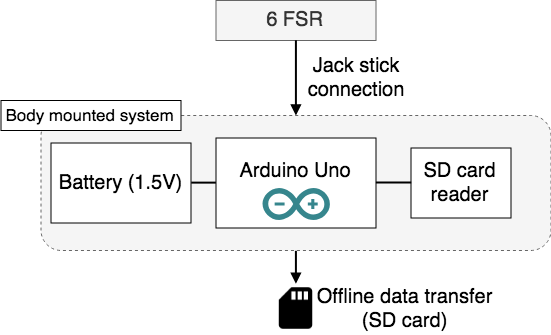
\includegraphics[width=.6\textwidth]{figures/circuitBoardSetup}
%	\caption{The setup of the Arduino-setup used for data collection from the FSRs on the feet. Collected data is saved on a microSD card and transferred offline to be processed on a computer with MATLAB.}
%	\label{fig:circuitBoardSetup}  %<--remember LABEL!
%\end{figure}

The system setup as a whole for both the gyroscope and FSR parts can be seen illustrated in a block diagram on \figref{fig:heleSystemSetup}.

\begin{figure}[H]
	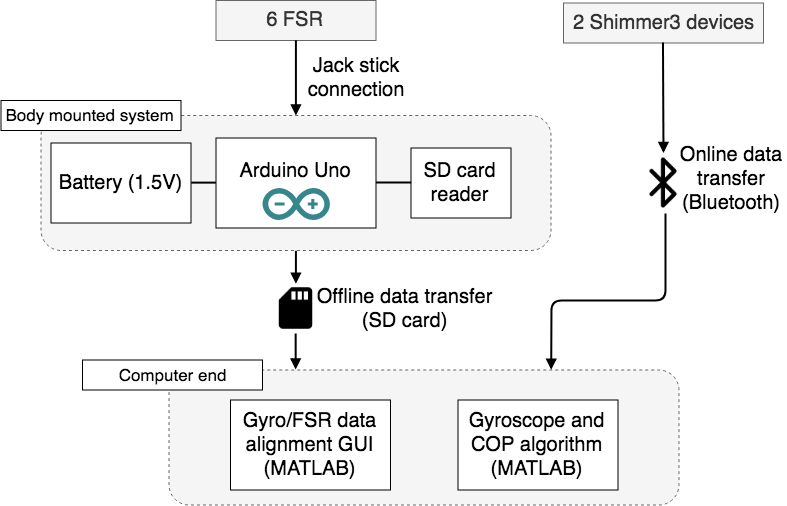
\includegraphics[width=.8\textwidth]{figures/heleSystemSetup}
	\caption{Block diagram of the system. The left side is of the pressure sensing part utilizing the FSRs. On the right side is the Shimmer3 devices (gyroscopes). All data is collected and processed on a computer using MATLAB.}
	\label{fig:heleSystemSetup}  %<--remember LABEL!
\end{figure}

\subsection{Instrumentation placement}

During data acquisition the subjects will be wearing the instruments presented earlier in \secref{methods:instrumentation}. The Shimmer3 devices will be placed, one on each leg, lateral distal to the knees of the subject.

The FSRs will be placed on the sole of each foot of the subject. One FSR 406 is placed at the lateral eminence of the sole. Of the two FSR 402 sensors, one will be placed under the heel and the other medial eminence of the sole. The placement of FSRs can be seen on \figref{fig:soleSensorPlacement}.

\begin{figure}[H]
	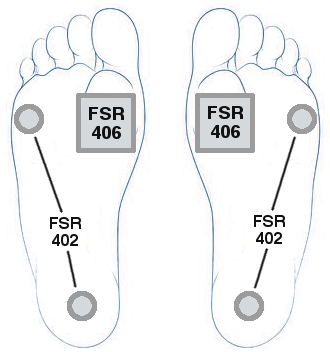
\includegraphics[width=.3\textwidth]{figures/humanSoleSensorPlacement}
	\caption{The placement of the FSR 402s and 406 under the foot of subjects.}
	\label{fig:soleSensorPlacement}  %<--remember LABEL!
\end{figure}

The Arduino-setup will be placed at the lower back of the subject and handle data collection. Collected data will be stored on an microSD card for offline analysis with MATLAB. An illustration of device placement on a subject can be seen in \figref{fig:bodySysSetup}.

%% SENSOR BAIT ALERT:
%jeg har skrevet at vi placere en FSR 406 (den store firkant sensor) under hælen. den skal sidde "bag" lilletåen.
%sensor bait tekst flyttet til bNEWSystemTest.tex

\begin{figure}[H]
	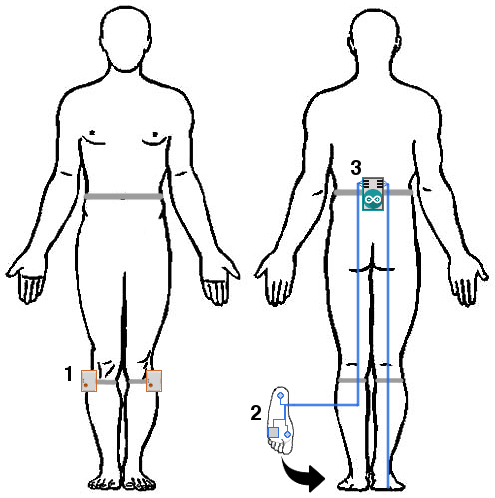
\includegraphics[width=.6\textwidth]{figures/bodySysSetup}
	\caption{The placement of the Shimmer3 IMU devices (1), FSRs under to feet (2) and Arduino-setup (3) on a test subject.}
	\label{fig:bodySysSetup}  %<--remember LABEL!
\end{figure}


